\chapter{Simulations à évènements discrets}
    \section{Introduction}
        Les simulations Monte Carlo présentées dans le chapitre précédent sont largement utilisées dans la modélisation de systèmes dans lesquels les entités (par exemple des clients, des tâches, des véhicules…) attendent leur tour pour accéder à un service ou une ressource limitée. Ces systèmes sont modélisés par des files d'attentes. La file d'attente est caractérisée par plusieurs paramètres, comme le taux d'arrivée des entités, la capacité de la file, la discipline de service (par exemple, premier arrivé, premier servi), et le taux de service. Dans les simulations Monte Carlo, ces caractéristiques sont représentées de manière stochastique, avec des temps d'arrivée et de service qui suivent des distributions de probabilité prédéfinies. Chaque itération de la simulation implique alors la génération de ces temps aléatoires, permettant de simuler le comportement de la file d'attente sous différents scénarios d'incertitude. Cela permet d'estimer des métriques de performance comme le temps moyen d'attente, la longueur moyenne de la file, et le taux d'utilisation des serveurs, qui sont essentiels pour optimiser les systèmes en file d'attente dans des domaines comme les télécommunications, les transports, et la gestion de stocks.
    
        \codeword{SimPy} (\cite{Simpy2023}), une bibliothèque Python orientée vers la simulation de processus discrets, permet de modéliser des entités (comme des machines, des clients, des événements) dans un système avec des routines qui évoluent au fil du temps. Pour y intégrer une simulation Monte Carlo, on peut utiliser des tirages aléatoires pour simuler l'incertitude dans les paramètres du système, comme les temps de service ou d'arrivée, et observer des milliers de scénarios différents. L’objectif est d’analyser les sorties d’un système en fonction de distributions probabilistes sur ces paramètres incertains.

    \section{File d'attente}
        \begin{definition}{Notation de Kendall}
            La notation de Kendall $A/S/C/K/m$ définit une \textbf{file d'attente}, où chaque paramètre spécifie certaines caractéristiques de la file. Le paramètre $A$ indique la loi de probabilité des instants d'arrivées, $S$ indique la loi de probabilité de la durée du service, $C$ indique le nombre de serveurs, $K$ est la capacité totale du système et $m$ indique la population totale de clients.
        \end{definition}
        Ce modèle de file est utilisé pour analyser des systèmes dans lesquels les arrivées sont aléatoires et indépendantes, le service est fourni par un unique serveur, et il n'y a pas de restriction de place pour la file d'attente. Le comportement de la file d'attente peut être analysé à l'aide de diverses métriques, telles que la probabilité d'avoir $n$ clients dans le système, le temps moyen dans la file et le nombre moyen de clients.

        \subsection{Simulation de file d'attente en Python}
            Comme expliqué précédemment, \codeword{SimPy} est une bibliothèque Python conçue pour la simulation de processus à événements discrets. Elle permet, notamment, de simuler des processus dans des systèmes stochastiques où les événements se produisent de manière aléatoire, comme dans les files d'attente. La modélisation de files d'attente est un excellent exemple d'application des simulations Monte Carlo, car elle repose sur des événements déclenchés par des arrivées et des départs aléatoires de clients, et les simulations Monte Carlo permettent d'étudier cet aspect aléatoire.

        \subsection{File d'attente à client unique}
            Le cas le plus trivial correspond au cas où un client arrive après un temps aléatoire, attend quelques secondes (dans l'exemple suivant, $5$), et puis repart. On remarquera que cette file d'attente est peut-être un peu trop simplifiée par rapport à la réalité. L'action de rentrer, attendre, et sortir peut être modélisée par un \texttt{processus}. En \codeword{SimPy}, ceci peut être modélisé par le code suivant:
            \inputminted{python}{codes/client_unique.py}
            On y a défini un \codeword{Environment}, dans lequel différents \textit{processus} peuvent avoir lieu. On y a défini une classe \codeword{Client}, contenant une seule méthode, \codeword{enter}. Notez l'utilisation du mot-clé \codeword{yield}: celui-ci est à la base de la notion de générateur\footnote{Testez, pour mieux comprendre l'utilisation de ce mot clé, le code suivant:
            \inputminted[fontsize=\tiny]{python}{codes/yield.py}}. Ainsi, la méthode \codeword{enter} définit un générateur, qui déclenche un \codeword{Event} après un temps défini par \codeword{timeout}. Lorsque cet évènement est déclenché, le client rentre, et un message s'affiche. À la ligne suivante, on produit un déclencheur après un second \codeword{timeout}. Lorsque le temps est écoulé, le client sort.
            La méthode \codeword{enter} est ajoutée à l'environnement en tant que processus au moyen de la fonction \codeword{env.process(func)}, appelée dans la méthode \codeword{__init__()}. Finalement, la simulation est lancée grâce à la ligne \codeword{env.run(until=t)}, où \texttt{t} est le temps total de simulation.
            
        \subsection{File d'attente à serveur unique}
            En \codeword{SimPy}, la notion de serveur peut être modélisée par un objet de type \codeword{Resource}. Une ressource est définie par une certaine capacité $c$, qui dans le cas d'un serveur unique, vaut $1$. Pas plus d'un client ne peut accéder à la ressource à la fois: les clients excédants doivent attendre que la ressource se libère pour y accéder. Le code suivant montre comment utiliser la notion de ressource:
            \inputminted{python}{codes/serveur_unique.py}

        \subsection{File d'attente à serveur multiple}
            Si l'on adapte le code précédent pour accepter une capacité $c>1$, alors la ressource peut être utilisée par plusieurs clients en même temps:
            \inputminted{python}{codes/serveur_multiple.py}

        \subsection{Statistiques de simulation}
            Nous savons maintenant réaliser des simulations de files d'attentes. Il est intéressant de récupérer diverses statistiques qui résultent de l'exécution des simulations. Le code suivant montre comment on peut récupérer le temps de service pour chaque client. Dans ce code, le temps de service est une variable aléatoire qui suit une loi exponentielle négative, parfois appelée \textit{loi Markovienne}. Pour cette raison, dans la notation de Kendall, la file modélisée est notée $M/M/2/\infty/5$.
            \inputminted{python}{codes/statistiques_de_service.py}
            Seulement, cette simulation ne nous donne le temps d'attente que de $5$ clients. Si l'on répète la simulation un grand nombre de fois, on peut ajouter à la liste contenant les mesures tous les temps de service de chacune des simulations et donner un aperçu bien plus informatif. Ce processus se nomme \textbf{simulation Monte Carlo}.
            \begin{definition}{Simulation Monte Carlo}
                La simulation Monte Carlo est une méthode numérique permettant d'estimer des solutions pour des problèmes complexes en générant un grand nombre de scénarios aléatoires. En modélisant les variables du système selon leurs distributions de probabilité, elle permet de produire des estimations statistiques sur les résultats d'intérêt.
            \end{definition}
            Le code peut alors être adapté: 
            \inputminted{python}{codes/statistiques_de_service_2.py} et le résultat est donné en figure \ref{fig:statistiques_de_service}. On voit clairement que les mesures suivent une loi exponentielle négative.
            \begin{figure}
                \centering
                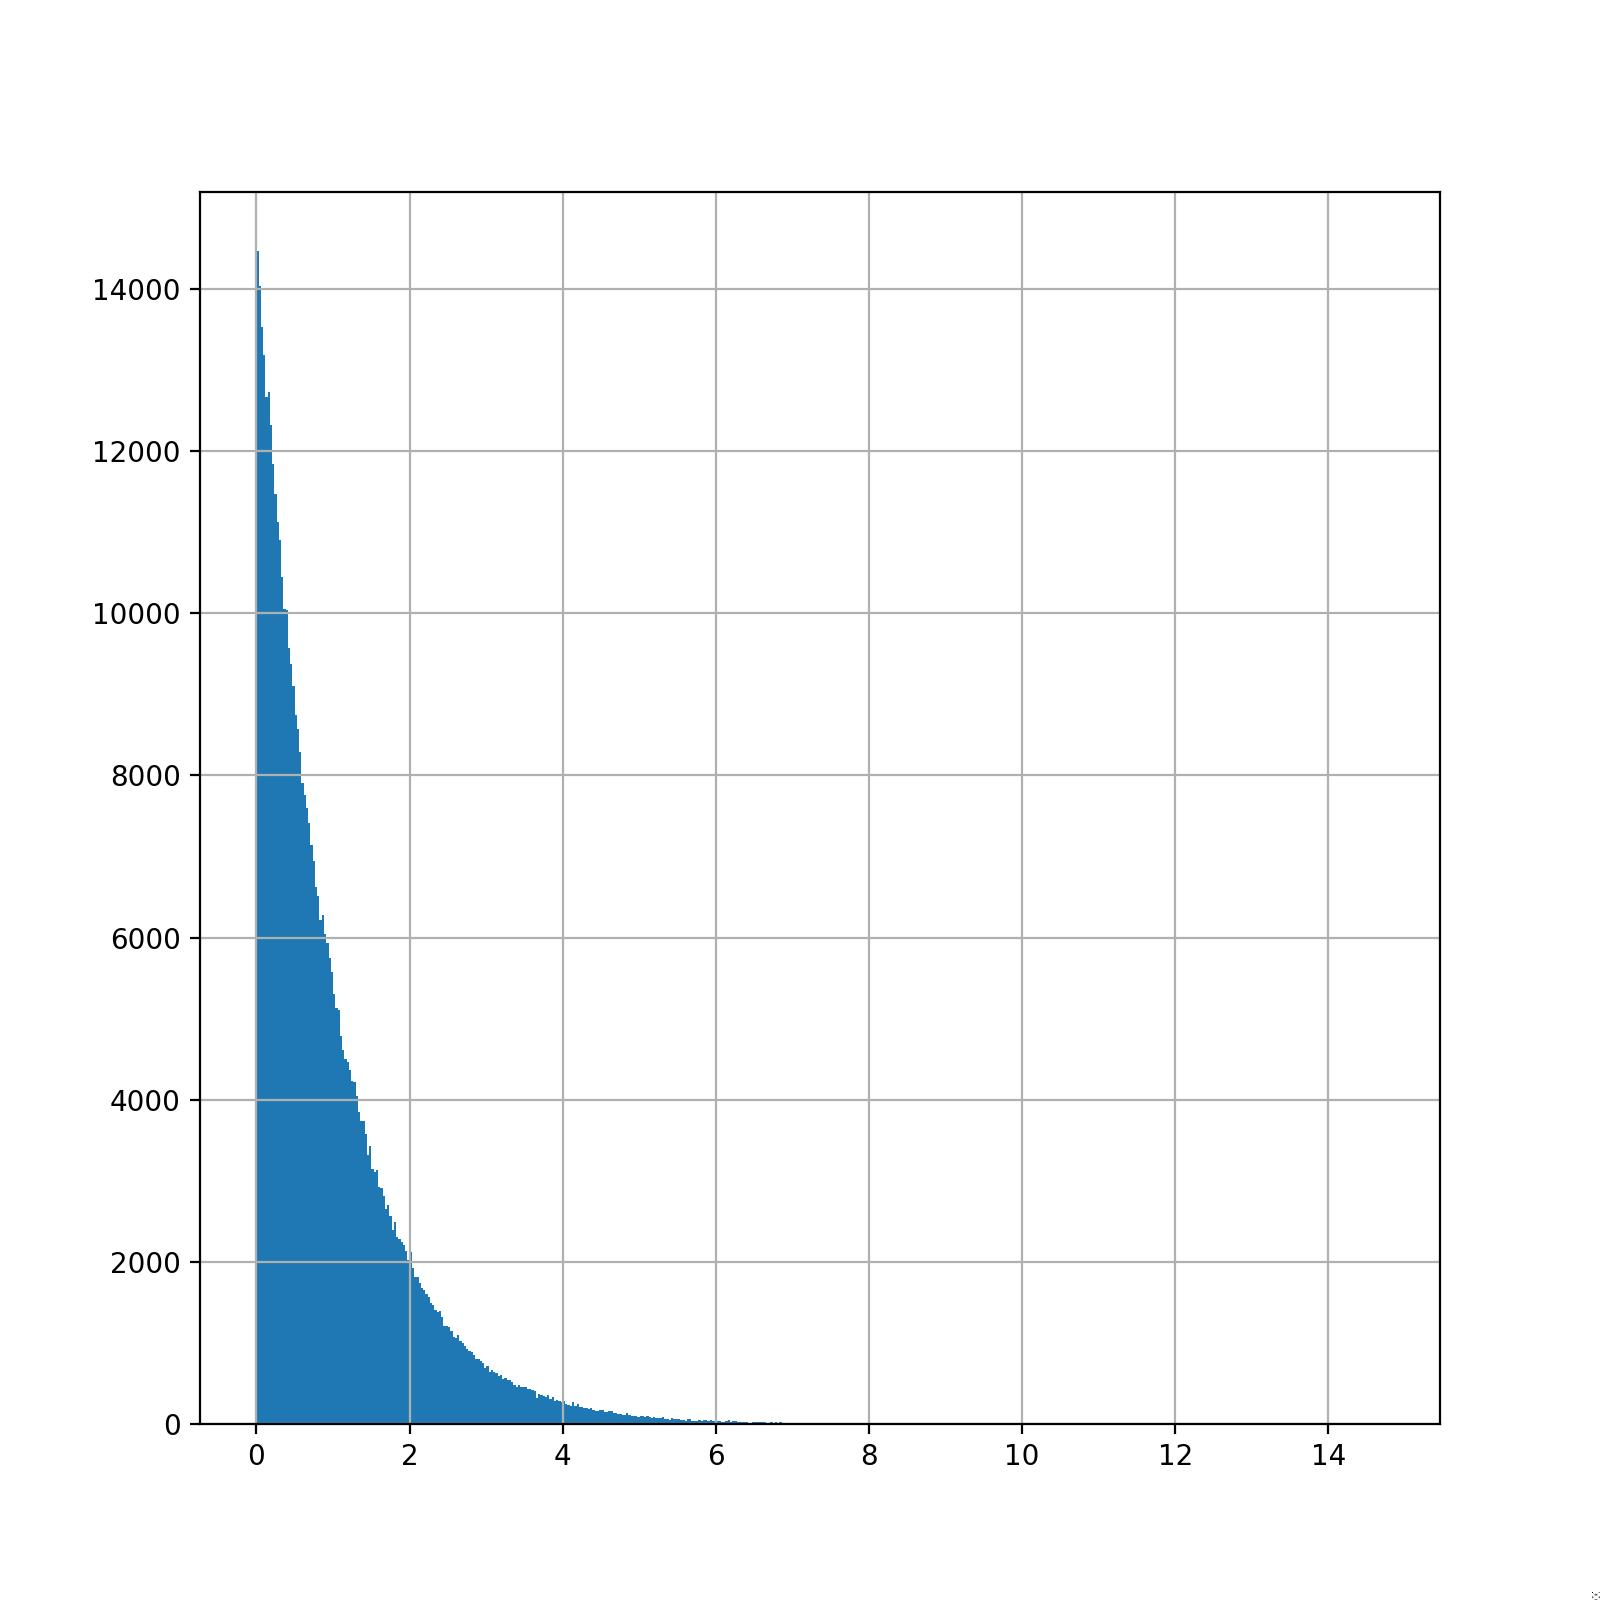
\includegraphics[width=\textwidth]{images/statistiques_de_service.jpg}
                \caption{Statistiques de service.}
                \label{fig:statistiques_de_service}
            \end{figure}
            
    \section{Exercice}
        On veut modéliser un service de charge de véhicules électriques. Le parc possède $4$ véhicules qui peuvent être loués de $8h$ à $22h$. Les véhicules ont une autonomie de $1h$ après lequel ils doivent être mis à charger jusqu'à charge complète. Le temps de charge $c$ suit une loi Markovienne de paramètre $\lambda = 1.5$. Les clients arrivent au magasin l'un après l'autre, avec un intervalle de temps les séparant qui suit une loi Markovienne de paramètre $\lambda = 0.2$. Ils louent un véhicule, si disponible, pour une durée qui suit une loi Markovienne de paramètre $\lambda=0.05$, et attendent sinon. 
        \begin{exercise}{Exercice 1}
            Formulez ce problème sous forme de file d'attente en suivant la notation de Kendall.
        \end{exercise}
        \begin{exercise}{Exercice 2}
            Modélisez la situation à l'aide de la librairie \codeword{SimPy}.
        \end{exercise}
        \begin{exercise}{Exercice 3}
            Déterminez, à l'aide d'une simulation Monte Carlo, la distribution et la moyenne du temps d'attente d'un client avant d'obtenir un véhicule.
        \end{exercise}
        \begin{exercise}{Exercice 4}
            Déterminez, à l'aide d'une simulation Monte Carlo, la distribution et la moyenne du nombre de recharges d'un véhicule.
        \end{exercise}

        Pour formuler le problème en utilisant la notation de Kendall, nous devons identifier les éléments suivants:
        \begin{itemize}
            \item type de la distribution d'arrivée des clients: les arrivées suivent une loi Markovienne marquée $M$~;
            \item type de la distribution du service (temps de location des véhicules) : le temps de location suit une loi Markovienne notée $M$~;
            \item nombre de serveurs (véhicules disponibles): $4$~;
            \item taille de la file d'attente: les clients attendent si aucun véhicule n'est disponible, donc la taille de la file d'attente est potentiellement infinie~;
            \item population : le nombre de clients potentiels est également supposé infini.
        \end{itemize}
        La notation de Kendall pour cette file d'attente est donc $M/M/4/\infty/\infty$.
        La solution aux exercices $2$, $3$ et $4$ est donnée dans le code
        \inputminted{python}{codes/charge.py}